% % % % % % % % % % % % % % % % % % % % % % % % % % % % % % % % % % % % % % % % % % % %
%                                                                                     %
% Short Sectioned Assignment LaTeX Template Version 1.0 (5/5/12)                      %
% This template has been downloaded from: http://www.LaTeXTemplates.com               %
%                                                                                     %
% Original author:  Frits Wenneker (http://www.howtotex.com)                          %
%                                                                                     %
% Modified by: Fco Javier Sueza Rodríguez (fcosueza@disroot.org)                      %
%                                                                                     %
% Changes:                                                                            %
%	    - Custom Chapters, Sections and Subsections (titlesec package)                %
%           - Document type scrbook (oneside)                                         %
%           - Use babel-lang-spanish package and marvosym                             %
%           - Use hyperref, enumitem, tcolorbox and glossaries packages               %
%           - Use Time New Roman (mathptmx), Helvetic and Courier fonts               %
%                                                                                     %
% License: CC BY-NC-SA 3.0 (http://creativecommons.org/licenses/by-nc-sa/3.0/)        %
%                                                                                     %
% % % % % % % % % % % % % % % % % % % % % % % % % % % % % % % % % % % % % % % % % % % %

%-----------------------------------------------%
%	              Packages                  %
%-----------------------------------------------%

\documentclass[paper=a4, fontsize=11pt, oneside]{scrbook}

% ---- Text Input/Output ----- %

\usepackage[T1]{fontenc}
\usepackage[utf8]{inputenc}
\usepackage{mathptmx}
\usepackage[scaled=.92]{helvet}
\usepackage{courier}
\usepackage[indent=12pt]{parskip}

\usepackage{geometry}
\geometry{verbose,tmargin=3cm,bmargin=3cm,lmargin=2.6cm,rmargin=2.6cm}

% ---- Language ----- %

\usepackage[spanish]{babel}
\usepackage{marvosym}

% ---- Another packages ---- %

\usepackage{amsmath,amsfonts,amsthm}
\usepackage{graphics,graphicx}
\usepackage{titlesec}
\usepackage{fancyhdr}
\usepackage{tcolorbox}
\usepackage{hyperref}
\usepackage{enumitem}
\usepackage[automake]{glossaries}

%--------------------------------------------------------------------%
%                      Customizing Document                          %
%--------------------------------------------------------------------%


% ----------- Custom Chapters, Sections and Subsections -------------- %

\titleformat{\chapter}[display]
			{\bfseries\Huge}
			{Tema \ \thechapter} {0.5ex}
			{\vspace{1ex}\centering}

\titleformat{\section}[hang]
			{\bfseries\Large}
			{\thesection}{0.5em}{}

\titleformat{\subsection}[hang]
			{\bfseries\large}
			{\thesubsection}{0.5em}{}

\titleformat{\subsubsection}[hang]
			{\bfseries\large}
			{\thesubsubsection}{0.5em}{}

\hypersetup{
    colorlinks=true,
    linkcolor=black,
    urlcolor=magenta
}

% ------------------- Custom heaaders and footers ------------------- %

\pagestyle{fancyplain}

\fancyhead[]{}
\fancyfoot[L]{}
\fancyfoot[C]{}
\fancyfoot[R]{\thepage}

\renewcommand{\headrulewidth}{0pt} % Remove header underlines
\renewcommand{\footrulewidth}{0pt} % Remove footer underlines

\setlength{\headheight}{13.6pt} % Customize the height of the header

% --------- Numbering equations, figures and tables ----------------- %

\numberwithin{equation}{section} % Number equations within sections
\numberwithin{figure}{section} % Number figures within sections
\numberwithin{table}{section} % Number tables within sections

% ------------------------ New Commands ----------------------------- %

\newcommand{\horrule}[1]{\rule{\linewidth}{#1}} % Create horizontal rule command


%----------------------------------------------------------------------------------------
%	TÍTULO Y DATOS DEL ALUMNO
%----------------------------------------------------------------------------------------

\title{
\normalfont \normalsize
\textsc{{\bfseries Curso 2022-2023} \\ Ciclo Superior de Desarrollo de Aplicaciones Web \\ IES Aguadulce} \\ [25pt]
\horrule{0.5pt} \\[0.4cm]
\huge Bases de Datos \\
\horrule{0.5pt} \\[0.4cm]
}

\author{Francisco Javier Sueza Rodríguez}
\date{\normalsize\today}

%----------------------------------------------------------------------------------------
%                                     DOCUMENTO
%----------------------------------------------------------------------------------------
\makeglossaries
\loadglsentries{glossary.tex}

\begin{document}

\maketitle

\newpage

\tableofcontents

\listoffigures

%\listoftables

\newpage

\chapter{Almacenamiento de la Información}
En este primer tema, vamos a estudiar los conceptos básicos sobre el almacenamiento de la información, así como de las bases de datos y los SGBD (Sistemas de Gestión de Bases de Datos), pero en primer lugar, vamos a hacer una introducción más detallada sobre que consideramos información y el contenido de este módulo.

\section{Introducción}
Si pensamos cualquier en cualquier aspecto de nuestra vida cotidiana, o si analizamos la mayoría de ámbitos de actividad, nos encontramos que la utilización de bases de datos esta ampliamente extendida. Estás, y los datos contenidos en ellas, serán imprescindibles para llevar a cabo multitud de acciones.

Algunas de las situaciones en las que es necesario el uso de bases de datos son las siguientes:

\begin{itemize}
    \item Cuando seleccionamos un canal de la TDT.
    \item Al utilizar la agenda del móvil para realizar una llamada telefónica.
    \item Cuando utilizamos un cajero automático.
    \item Cuando acudimos a la consulta del médico.
    \item Al inscribirnos en un curso, plataforma online, etc...
    \item Si utilizas el GPS.
    \item Cuando reservamos unas localidades en un evento deportivo.
    \item Cuando consultamos cualquier información en internet.
    \item Al solicitar un certificado de un organismo oficial.
\end{itemize}

Como vemos, el gran volumen de datos que manejamos y sus innumerables posibilidades hacen necesaria la existencia de técnicos perfectamente formados y capaces de trabajar con ellos.

Este módulo profesional se centra, precisamente, en las \textbf{Bases de Datos} y su uso en el desarrollo de aplicaciones. En esta primera unidad, comenzaremos conociendo los primeros sistema basados en ficheros para el almacenamiento y gestión de la información.  Seguidamente, se desarrollarán los conceptos y definiciones básicas relacionados con las bases de datos, viendo también sus modelos y tipos. Más adelante conocer los sistemas gestores de bases de datos y finalmente, veremos las herramientas reales con las que llevar a caso dicha gestión.

\section{Los Ficheros de Información}
En esta sección vamos a hablar de los fichero de información, en que consiste, que tipos nos podemos encontrar, métodos de acceso y parámetros de utilización.

\subsection{¿Que es un Fichero?}
En la década de los setenta, los procesos básicos relacionados con una empresa se centraban en la contabilidad y facturación. Las necesidades de almacenamiento y gestión de la información podían satisfacerse con un número relativamente reducido de archivos de papel agrupados y ordenados, los típicos ficheros clásicos.

Con la primera informatización, se paso del papel al ordenador, pudiendo acceder a los datos de forma mucho más rápida. Los ordenadores adaptaron sus herramientas para que se asemejaran a las que los usuarios utilizaban manualmente, de forma que en informática también empezó a hablarse de ficheros, carpetas, formularios, etc...

La información que empezó a tratarse en los ordenadores debía ser almacenada para su posterior recuperación, consulta y procesamiento. El elemento que se creo para almacenar esta información fue el \textbf{fichero} o \textbf{archivo}.

Podemos definir un \textbf{fichero} como el \textbf{conjunto de información relacionada}, tratada como un todo y organizada de \textbf{forma estructurada}. Es una secuencia de  dígitos binarios que organiza información relacionada con el mismo aspecto.

Los fichero están formados por \textbf{registros lógicos} que contienen información relativa a un mismo elemento u objeto (por ejemplo, información de un usuario). A su vez, los registros están divididos en \textbf{campos} que tienen cada una de las informaciones elementales que forman un registro (por ejemplo, nombre de usuario, email,...).

Los datos están almacenados de forma que se pueda añadir, suprimir, actualizar y consultar, individualmente, en cualquier momento.

Como los ficheros suelen ser muy grandes, solo se puede llevar parte de ellos a la memoria principal para procesarlos. La cantidad de información que es transferida entre el soporte en el que se almacena el fichero y la memoria del ordenador, en solo una operación de lectura/escritura, se llama \textbf{registro físico} o  \textbf{bloque}.

Normalmente en cada operación de lectura/escritura se transfieren varios registros de un fichero, es decir, un bloque suele contener varios registros lógicos. Al número de registros que entran en un bloque se le llama \textbf{factor de blocaje}, y a la operación de agrupar varios registros en un mismo bloque se conoce como \textbf{bloque de registros}.

\subsection{Tipos de Ficheros}
Según la función que vaya a desempeñar un fichero, estos pueden ser clasificados de varias maneras:

\begin{enumerate}[label=(\alph*)]
    \item \textbf{Ficheros Permanentes}: contiene información relevante para una aplicación. Es decir, los datos necesarios para el funcionamiento de ésta. Tiene un período de permanencia en el sistema amplio. Se subdividen en:
    \begin{itemize}
        \item \textbf{Ficheros Maestros}: contiene el estado actual de los datos que pueden modificarse desde la aplicación. Es la parte central de aplicación, su núcleo.
        \item \textbf{Ficheros Constantes}: son aquellos que incluyen datos fijos de la aplicación. No suelen ser modificados y se accede a ellos para la realización de consultar.
        \item \textbf{Ficheros Históricos}: contiene datos que fueron considerados como actuales en un período o situación anterior. Se utilizan para la reconstrucción de situaciones o estados concretos.
    \end{itemize}

    \item \textbf{Ficheros Temporales}: se utilizan para almacenar datos que son útiles para un parte de la aplicación. Son generados a partir de datos de ficheros permanentes y tienen un período corto de existencia. Estos pueden ser:
    \begin{itemize}
        \item \textbf{Ficheros Intermedios}: almacenan resultados de una aplicación que serán usados por otra.
        \item \textbf{Ficheros de Maniobras}: almacenan datos de una aplicación que no pueden ser mantenidos en memoria por falta de espacio.
        \item \textbf{Ficheros de Resultados}: almacenan datos que van a ser transferidos a un dispositivo de salida.
    \end{itemize}
\end{enumerate}

En la siguiente figura podemos ver un esquema con esta clasificación.

\begin{figure}[ht]
    \centering
    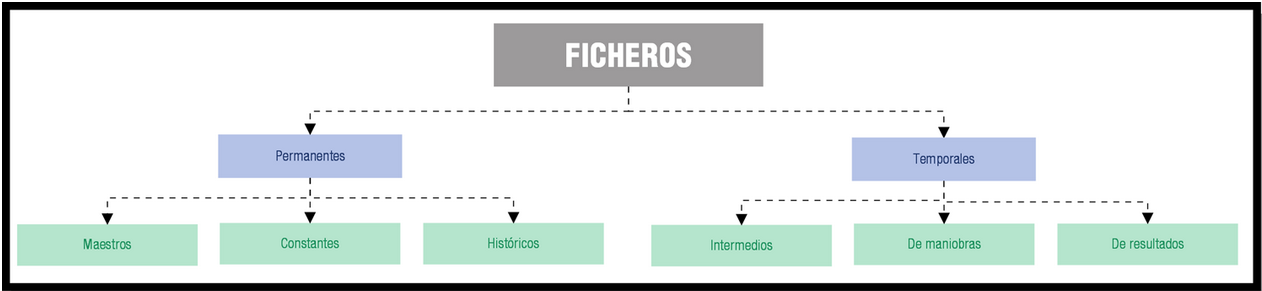
\includegraphics[scale=0.35]{ficheros-tipos.png}
    \caption{Clasificación de ficheros según su función}
\end{figure}

\subsection{Los Soportes de la Información}
Los ficheros se almacenan en soportes de información manejados por periféricos del ordenador, que permiten leer y grabar datos en el soporte. Los soportes más utilizados son las \textbf{cintas magnéticas} y los \textbf{discos} (magnéticos, ópticos o magneto-ópticos).

Al principio se usaban tambores de cinta magnética, similares en tamaño a un disco de vinilo, funcionaban de manera similar a los antiguos casetes, pero al tener un tamaño mucho más grande permitían almacenar mucha mas información, permitiendo el acceso a esta de forma secuencia.

Posteriormente los medios de almacenamiento fueron evolucionando a la par que el hardware, en concreto con la aparición de los disquetes y el disco duro. Estos dispositivos ya permitían el acceso aleatorio a los datos.

Por lo tanto, podemos distinguir dos tipos de dispositivos de almacenamiento de datos:

\begin{itemize}
    \item \textbf{Soportes de Acceso Directo a Datos}: son los más empleados y el acceso a datos se hacer de forma directa, pudiendo colocarlos en la posición que más nos interese.
    \item \textbf{Soporte de Acceso Secuencial}: se suele usar en copias de seguridad y si deseamos leer un dato que esta a mitad de la cinta, tendremos que leer todo lo que hay hasta llegar a esa posición.
\end{itemize}

% Glossary

\glsaddall
\printglossaries

% Bibliography

\newpage
\addcontentsline{toc}{chapter}{Bibliografía}
\bibliography{citas}
\bibliographystyle{unsrt}

\end{document}